% =============================================================================
% DOCUMENTO .tex QUE PERMITE COMPILAR EL TRABAJO FINAL DE ASIGNATURA ALTA CAPACIDAD EN PDF
% Máster Universitario en Formación del Profesorado =============================================================================

\documentclass[12pt, a4paper]{article}


% --- Paquetes de Idioma y Codificación ---
\usepackage[utf8]{inputenc}
\usepackage[T1]{fontenc}
\usepackage[spanish, es-tabla]{babel}

\usepackage{placeins} % para usar FloatBarrier
\usepackage{graphicx} % para usar figure
\usepackage{caption} % mejora compatibilidad con captions

\usepackage{pdfpages} % Para incluir la declaración jurada de autoria (que chupa en PDF generado por adobescan).

\usepackage[most]{tcolorbox} % per fer shadeboxes

\usepackage{xurl} % permet barres baixes a les url



% --- Tipografía similar a Times New Roman ---
\usepackage{newtxtext,newtxmath} 

% permite definir espacios customizados en 
% un begin itemize.
\usepackage{enumitem}

% --- Configuración de Márgenes (Normativa académica estándar) ---
\usepackage{geometry}
\geometry{
	a4paper,
	top=30mm,
	bottom=30mm,
	left=35mm,
	right=35mm
}

% --- Tipografía y Espaciado ---
\usepackage{setspace}
\onehalfspacing % Interlineado 1.5 (para satisfacer normativa UNED)
\usepackage{parskip} % Espaciado automático entre párrafos sin sangría excesiva

% --- Gestión de Bibliografía (APA 7ª Edición) ---
\usepackage{csquotes}
\usepackage[style=apa, backend=biber, language=spanish]{biblatex}

% --- Enlaces y Marcadores PDF ---
\usepackage{hyperref}
\hypersetup{
	colorlinks=true,
	linkcolor=blue,        
	filecolor=magenta,      
	urlcolor=blue,
	citecolor=black,        
	pdftitle={TrabajoObligatorioOrientacionInclusivaAACC},
	pdfauthor={Santiago Sánchez Sans}
}

\addbibresource{bibliografia.bib}

% =============================================================================
% PORTADA DEL DOCUMENTO (Configuración UNED)
% =============================================================================
%SE HA ANONIMIZADO TODO POR QUE LA SUBIDA A GITHUB ES PÚBLICA!
\title{
	\vspace*{-2cm} % El asterisco fuerza el espacio al inicio de la página
	\textbf{\Large UNIVERSIDAD NACIONAL DE EDUCACIÓN A DISTANCIA (UNED)}\\[0.5cm]
	\large FACULTAD DE EDUCACIÓN\\[1.5cm]
	\LARGE \textbf{Orientación Inclusiva en las Necesidades Educativas Asociadas a Factores Socioculturales y a la Alta Capacidad (trabajo obligatorio)}\\[0.4cm]
	\large 
	\vspace{1cm}
	Máster Universitario en Formación del Profesorado de Educación Secundaria Obligatoria y Bachillerato, Formación Profesional y Enseñanza de Idiomas
	\vspace{2cm} % Sustituido el salto de línea \\ por \vspace normal
}

\author{
	\textbf{Autor/a:} Santiago S.S. $|$ \textbf{DNI:} ANÓNIMO \\[0.2cm]
	\textbf{teléfono:} anónimo $|$ \textbf{e-mail:} anónimo@gmail.com\\[0.2cm]
	\textbf{Especialidad:} anónimo\\[0.2cm]
	\textbf{Centro Asociado:} anónimo
	% Eliminado el \\[0.2cm] final que causaba error de salto de línea
}

\date{\vfill Curso Académico: 2025/2026\\ \vspace{0.5cm} Convocatoria: Septiembre 2026 (entrega: 01/09/2026)}

% =============================================================================
% CUERPO DEL DOCUMENTO
% =============================================================================
\begin{document}
	
	\maketitle
	\thispagestyle{empty} % Elimina numeración en la portada
	\newpage
	
	% --- Índice ---
	\pagenumbering{arabic} % Numeración romana para el índice y preliminares
	\tableofcontents
	\newpage
	
	\pagenumbering{arabic} % Con la "R" mayúscula numeración romana!
	\setcounter{page}{1}
	
	% --- Parte 1: preliminares ---
	\section{Preliminares}
	
	
	\subsection{Declaración jurada de autoría}
	% PENDENT A DESCOMENTAR!
	\includegraphics[width=\textwidth]{img/declaracioJuradaAutoria_NoGithub.pdf}
	\subsection{Explicación general de cómo se ha realizado el trabajo}
	\label{sec:explicGeneral}
	
	Para empezar el documento se ha realizado utilizando un procesador de textos y un gestor de bibliografía diferentes a microsoft word. Se ha usado LaTeX para escribir esta memoria (este es el archivo \href{https://github.com/santiUNED/orientacionInclusivaAACC/blob/main/main.tex} {main.tex} que escribí para crearla) y y este es el archivo bibtex que el programa .tex utiliza para gestionar la bibliografía (\href{https://github.com/santiUNED/orientacionInclusivaAACC/blob/main/bibliografia.bib}{bibliografia.bib}). LaTeX es un compilador de textos \textit{open-source} o de código abierto que toma un código en extensióm.tex, escrito a modo de lenguaje de marcas, y en el proceso de compilación genera un PDF con una tipografía y una calidad excelentes.
	
	Este es el sistema que utilicé para realizar un trabajo de fin de máster en 2017 (\href{https://drive.google.com/file/d/1axwlOY0EuuCQX0HfZH30yWjXO3ruYdS0/view}{link}) y el sistema que usé para la memoria del trabajo final de un grado superior en 2025 (\href{https://drive.google.com/file/d/12gHzV9FWSaKpbUgoN8VF0Hd1BpAlayGW/view}{link}). Estoy familiarizado con él y lo conozco ya muchísimo más que word, así que tomé la decisión de usarlo.
	
	Una de las dificultades es que no ha sido posible utilizar la tipografía Arial, ya que LaTeX no la incluye.
	
	Se ha utilizado el comando \verb|\textcite{gagneModelBasatEnRendiment}| para generar  citas en texto ``\textcite{gagneModelBasatEnRendiment}'' y el comando \verb|\parencite{gagneModelBasatEnRendiment}| para conseguir lo propio con las citas parénticas del estilo ``\parencite{gagneModelBasatEnRendiment}''. La compilación se ha hecho usando el editor de código online overleaf (\href{https://www.overleaf.com/}{(link)} y la librería ``csquotes'' que, llamada mediante estos comandos en la cabecera del archivo .tex, permite hacer citaciones en estilo APA de forma autimatizada.
	
	\begin{center}
		\small
		\verb|\usepackage{csquotes}|
		\verb|\usepackage[style=apa, backend=biber, language=spanish]{biblatex}|
	\end{center}
	
	Algunas referencias bibtex se han obtenido de la base de datos Scopus directamente (figura \ref{fig:gagneSCPbib}) y otras de research gate (figura \ref{fig:gagneRGbib}).
	
	\FloatBarrier
	\begin{figure}[htbp]
		\centering
		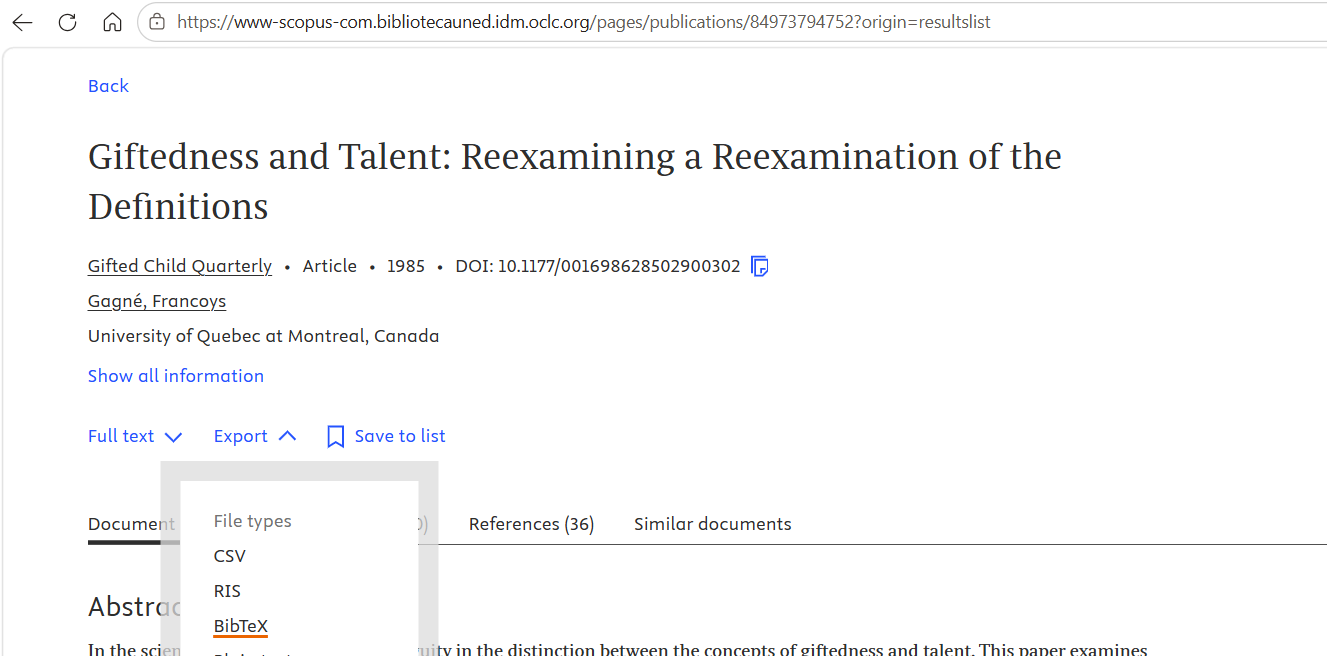
\includegraphics[width=1\textwidth]{img/gagneScopusBIB.png}
		\caption{Obtención de una referencia bibliográfica en formato .bib (bibtex) a través de Scopus usando la red de la UNED.}
		\label{fig:gagneSCPbib}
	\end{figure}
	\FloatBarrier
	
	\FloatBarrier
	\begin{figure}[htbp]
		\centering
		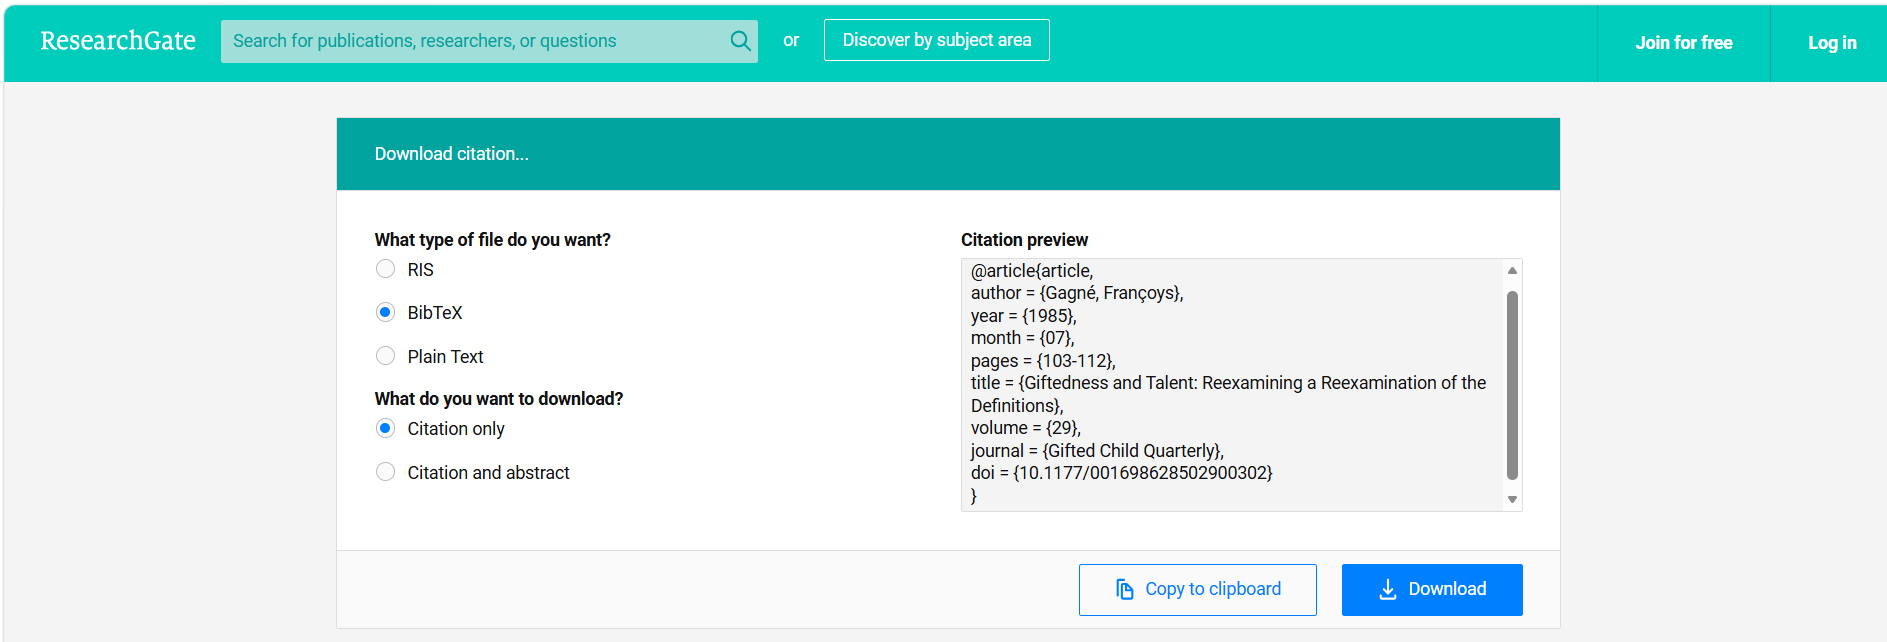
\includegraphics[width=1\textwidth]{img/gagneResearchGateBIB.png}
		\caption{Obtención de una referencia bibliográfica en formato .bib (bibtex) a través de reserarch gate}
		\label{fig:gagneRGbib}
	\end{figure}
	\FloatBarrier
	
	
	
	
	
	
	La misma base de datos Scopus permite descargar las referencias bibliográficas y, a veces, la semilla .bib para la bibliografía la obtuve de aquí. Por ejemplo, para acceder a la fuente primaria del modelo diferenciado de dotación y talento \parencite{gagneModelBasatEnRendiment}, fue necesario acceder al full text mediante scopus (ver figura \ref{fig:scopusGagneImatge}) y también obtuve de ahí la bibliografía.
	
	\FloatBarrier
	\begin{figure}[htbp]
		\centering
		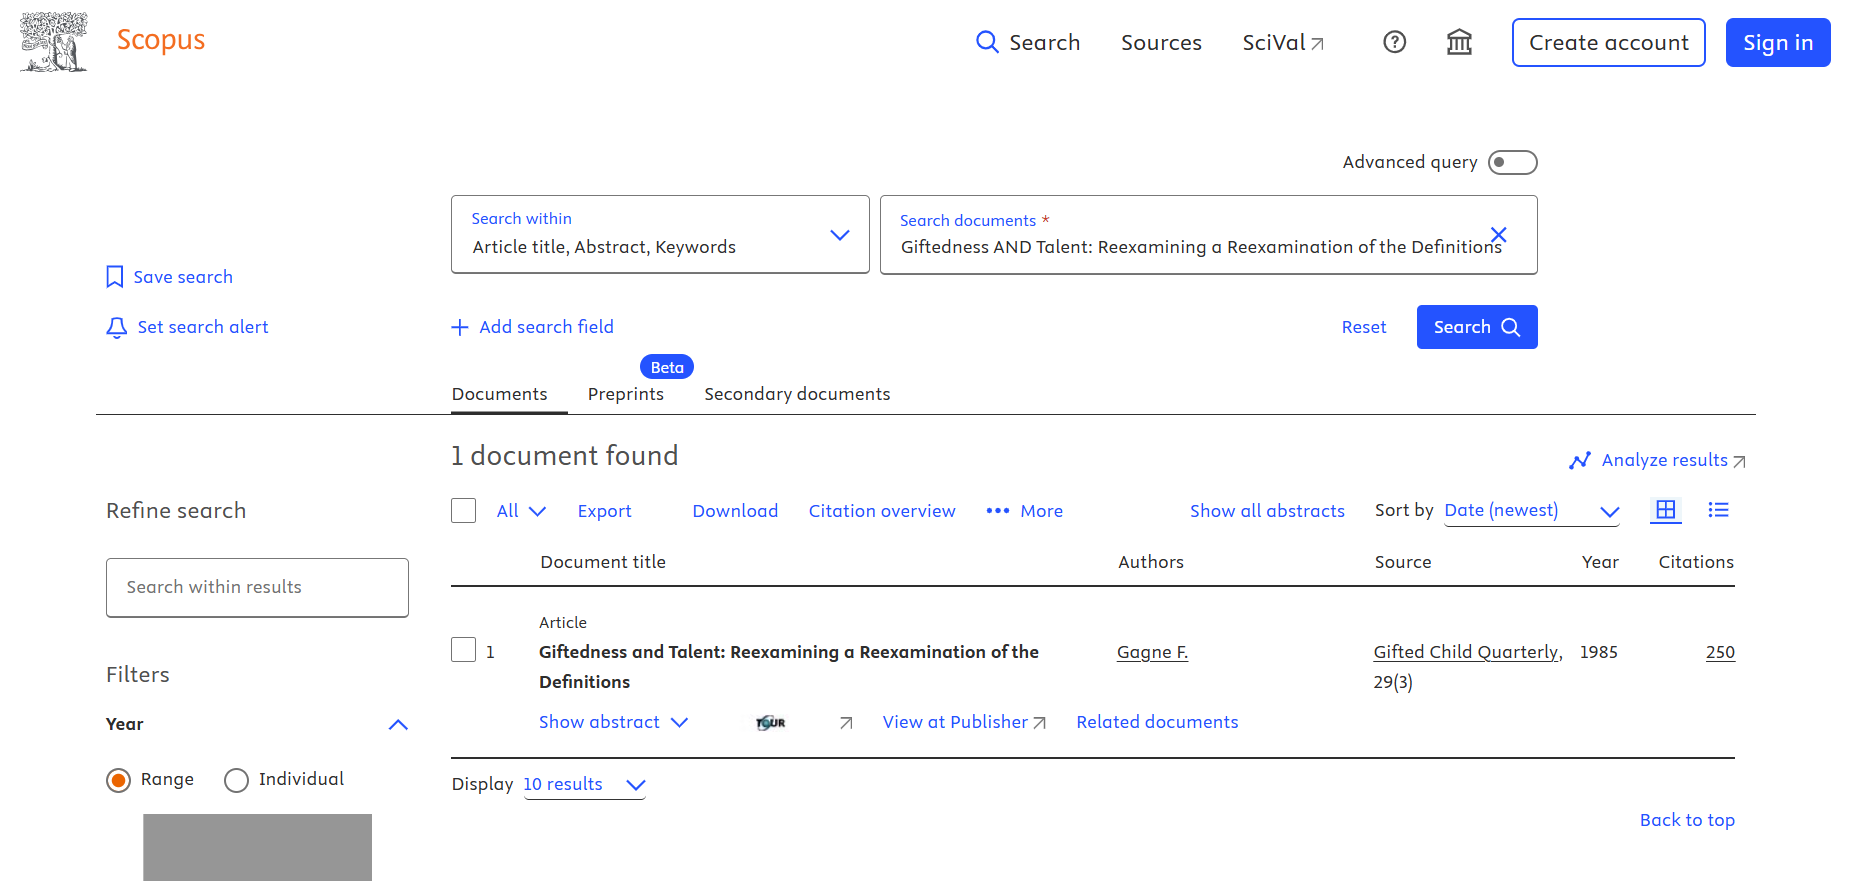
\includegraphics[width=1\textwidth]{img/scopusGagne.png}
		\caption{Búsqueda en Scopus del full text del modelo de Gagné, no accesible sin usar los recursos electrónicos de la UNED.}
		\label{fig:scopusGagneImatge}
	\end{figure}
	\FloatBarrier
	
	
	La creación de texto no incluye ningún uso de IA. Todas las frases que llegará a leer el lector de este trabajo han sido escritas por mi o se han parafraseado de otros autores, quedando con todas sus imperfecciones e idiosincracias. El uso de la inteligencia artificial, empero, no ha sido nulo: sí ha sido utilizado para ayudarse con la gestión de la bibliografia en los casos en los que la sintaxis necesaria para escribir fragmentos del archivo .bib no se pudiese extraer directamente de Scopus o de research gate (que tienen sistemas que la extraen automáticamente); asimismo, la IA se ha utilizado para generar fragmentos de código del lenguaje de marcas que permite compilar a PDF.
	
	También se usó Scopus para tratar de encontrar referencias primarias. Esta fue la sintaxi usada para encontrar un estudio de Gardner que sabía que databa de 1983 (figura \ref{fig:gardnerIntent}).
	
	
	\FloatBarrier
	\begin{figure}[htbp]
		\centering
		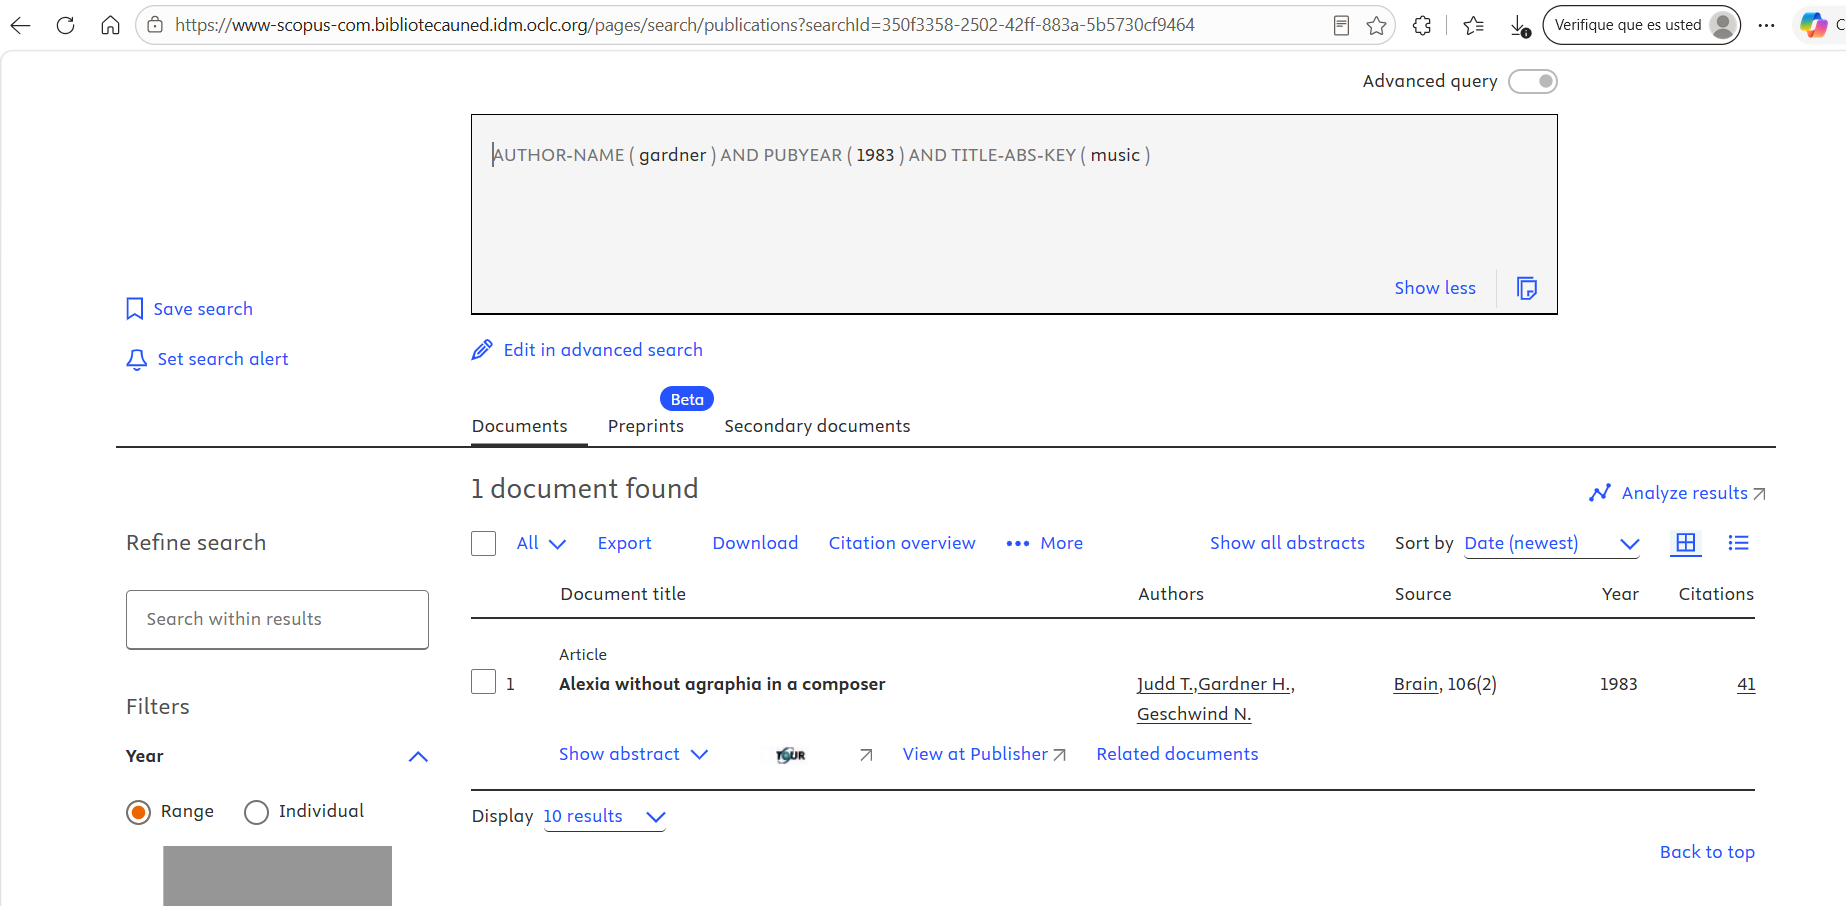
\includegraphics[width=.9\textwidth]{img/CercaGardner1983.png}
		\caption{Búsqueda específica de un estudio de Gardner, datado del año 1983,}
		\label{fig:gardnerIntent}
	\end{figure}
	\FloatBarrier

	
	Para entender un flujo de trabajo normal de trabajo en el que interviene la IA en mi trabajo, podéis ver la figura \ref{fig:explicacioGimpLatex}, donde se puede ver primero como edito una imagen en gimp, como luego renderizo esa misma imagen correctamente en el documento pdf, y como previamente la IA me ha creado un esqueleto con el lenguaje de marcas necesario que permite crear la compilación a pdf.
	
	
	
	\FloatBarrier
	\begin{figure}[htbp]
		\centering
		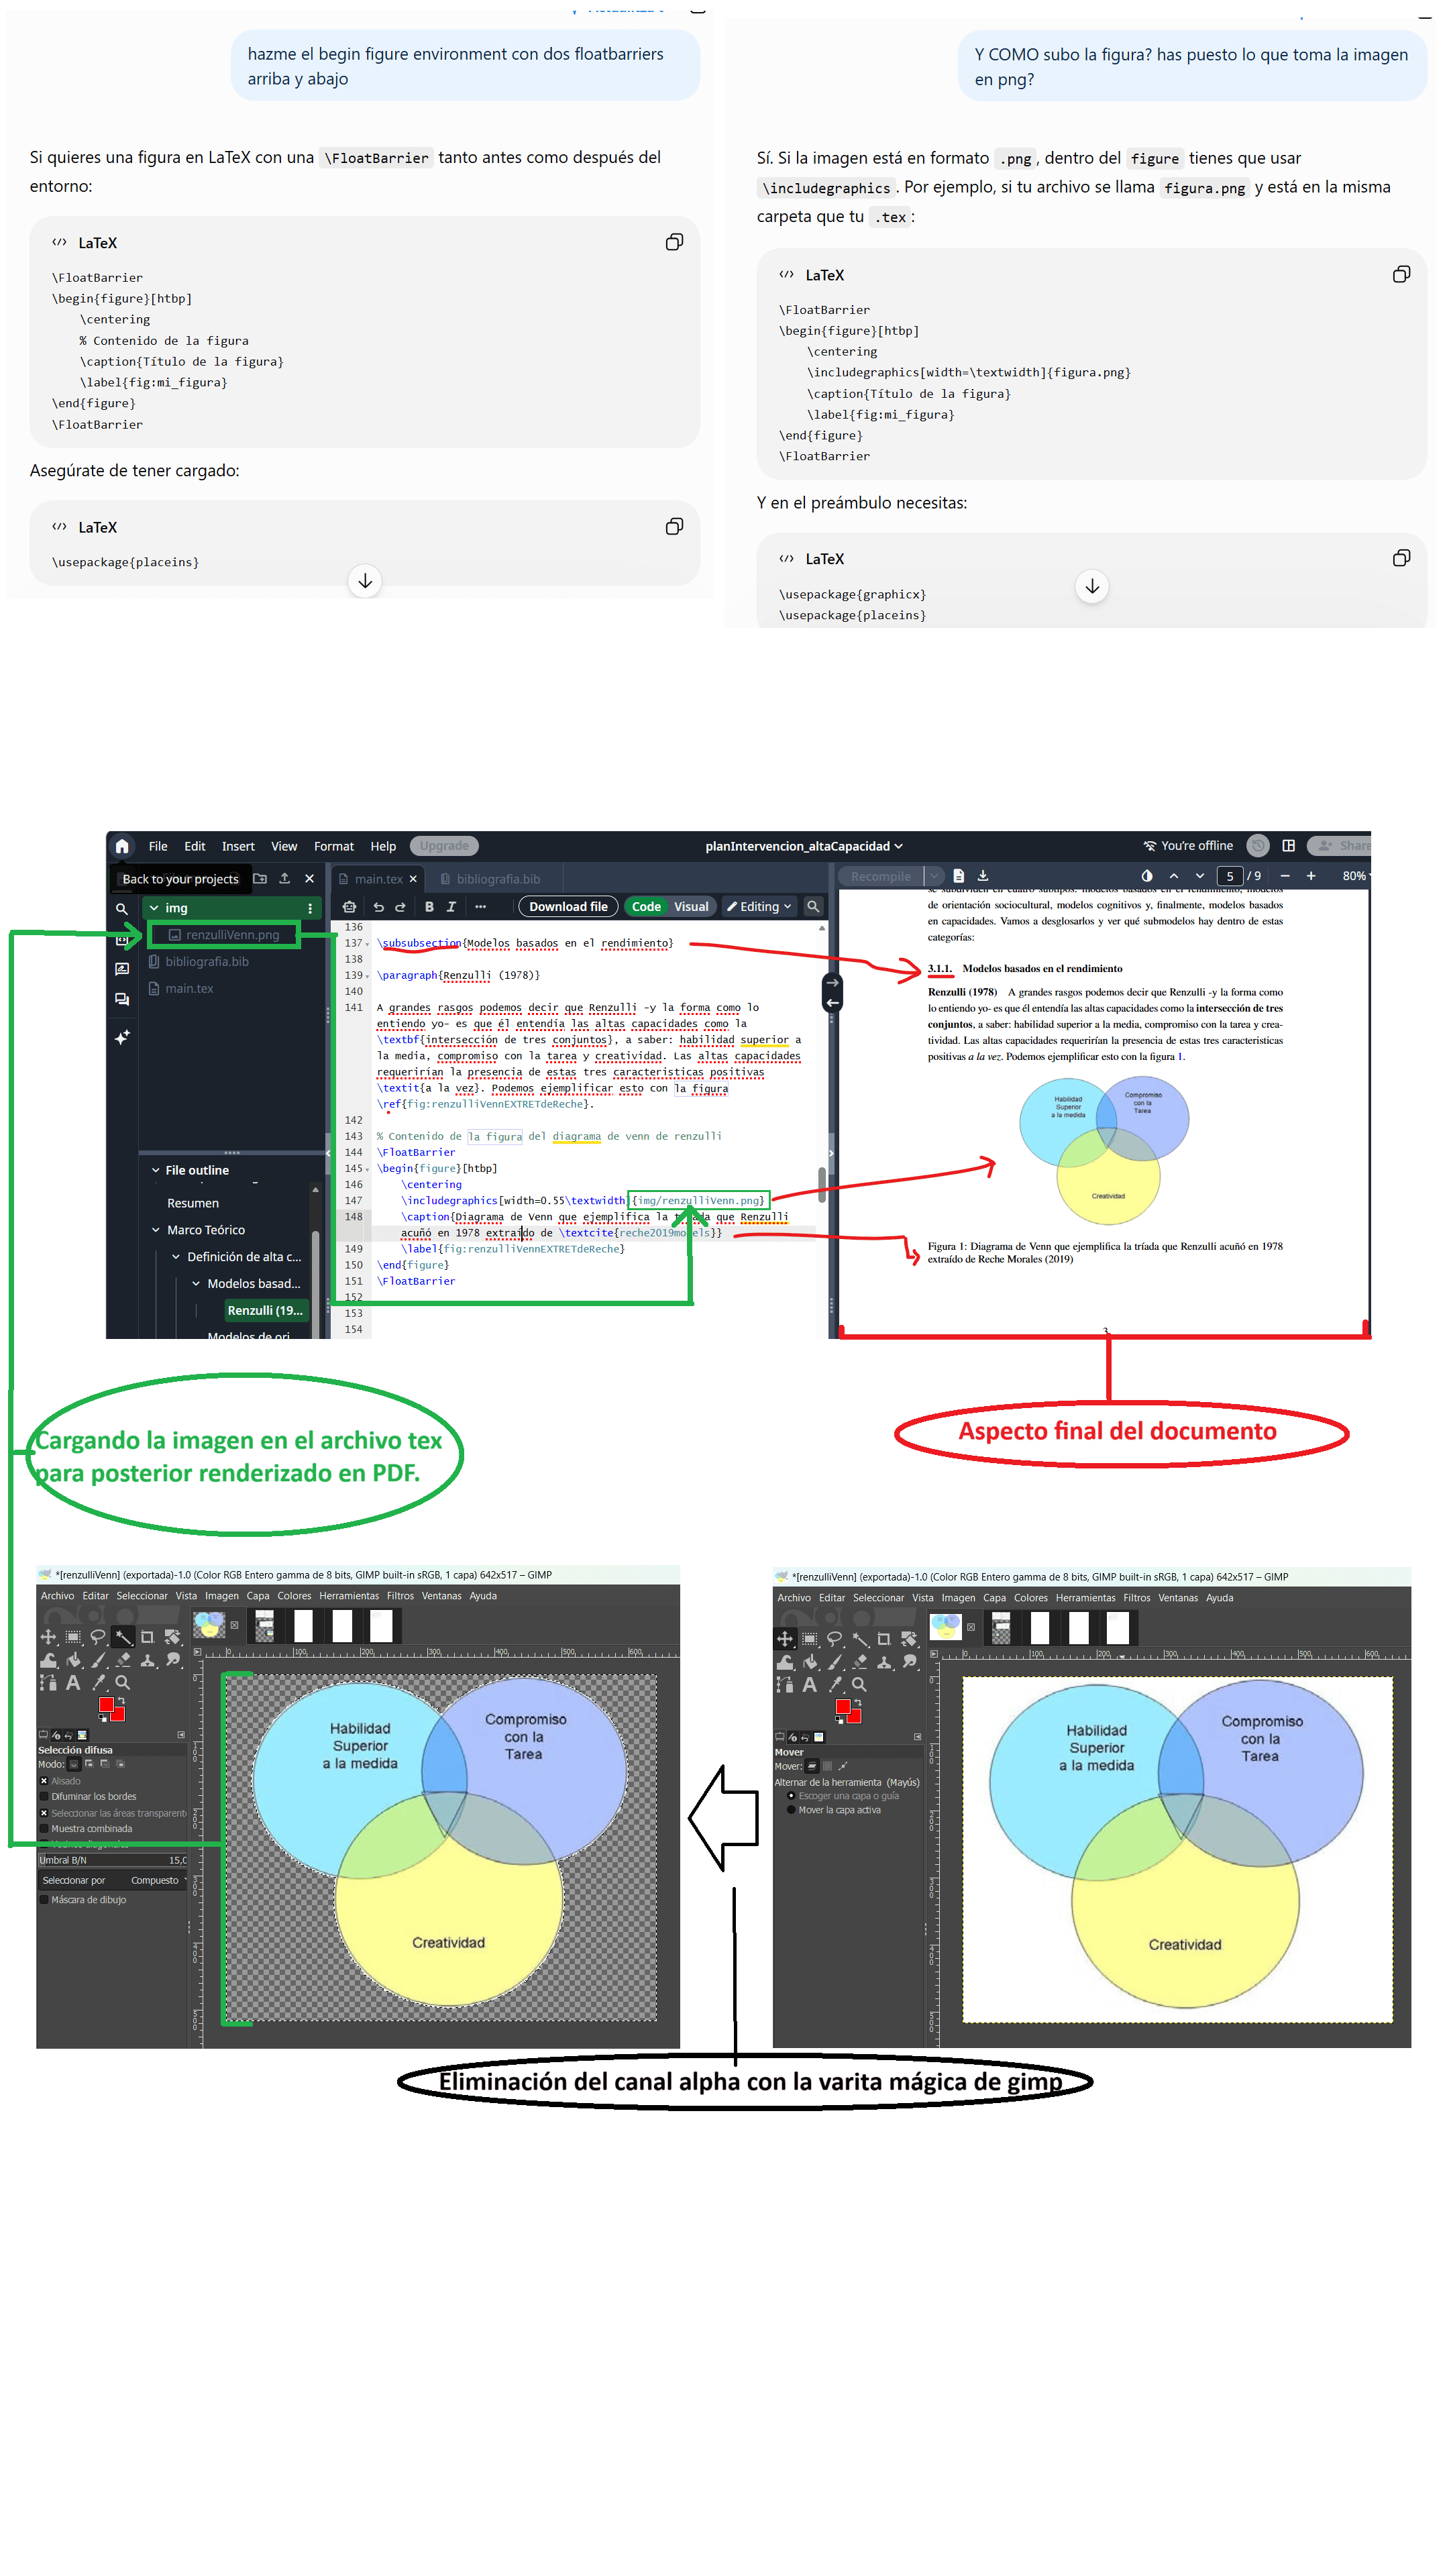
\includegraphics[width=.9\textwidth]{img/explicacioIAgimpLatexV2.png}
		\caption{Addición de una imagen con LaTeX, asistido por IA}
		\label{fig:explicacioGimpLatex}
	\end{figure}
	\FloatBarrier
	
	
	
	
	
	% --- Parte 2: el abstract ---
	\newpage
	\section{Resumen}
	
	\textit{Texto de entre 200 y 250 palabras exponiendo el objetivo del trabajo, la metodología utilizada y las principales conclusiones de la intervención.}
	
	El objetivo de este trabajo es aprender los modelos teóricos para conceptualizar la sobredotación intelectual en alumnos de nuestro ámbito de actuación (principalmente la ESO, pero también en la enseñanza postobligatoria no universitaria). Asimismo, se pretende conocer los protocolos de actuación de la comunidad autónoma para el abordaje de un plan de intervención y atención a las altas capacidades, y volcar estos objetivos en la resolución de un caso de altas capacidades, valorando propuestas de intervención, los roles del orientador y los recursos necesarios para su correcta intervención.
	
	Para ello, en primer lugar se ha realizado una revisión de los principales modelos teóricos de las altas capacidades, incluyendo los modelos basados en el rendimiento, los modelos socioculturales, los modelos cognitivos y los modelos basados en capacidades.
	
	A continuación, se ha estudiado el marco normativo y los protocolos de actuación en Cataluña, prestando especial atención al proceso de detección, evaluación psicopedagógica y derivación al EAP, así como a las medidas educativas que pueden aplicarse. Finalmente, estos conocimientos se han aplicado al análisis de un caso práctico de un alumno de 1.º de ESO con altas capacidades, planteando una propuesta de evaluación e intervención ajustada a sus características. La actividad ha permitido comprender la importancia de conocer tanto los fundamentos teóricos como los procedimientos a nivel de comunidad autónoma, para realizar una intervención educativa adecuada al marco de trabajo actual y futuro del aspirante al máster.


	
	
	% --- Parte 3: Marco Teórico (3-5 páginas)
	\newpage
	\section{Marco Teórico}
	
	
	\subsection{Definición de alta capacidad y modelos teóricos existentes.}
	
	De acuerdo con el glosario de esta asignatura se define a un \textit{alumno con alta capacidad} como aquel ``Alumno que aprende a mayor ritmo, con mayor profundidad y mayor amplitud que sus iguales, sobre todo si trabaja con desafíos adecuados a su capacidad y si encuentran en familia y profesores el estímulo y la guía adecuados. La alta capacidad precisa del contexto para materializarse'' \parencite{unedGlossariAltaCapacitat}. \textcite{reche2019models}, nos conceptualiza que los modelos explicativos de alta capacidad se subdividen en cuatro subtipos:\textit{ modelos basados en el \textbf{rendimiento}, modelos de \textbf{orientación sociocultural}, modelos \textbf{cognitivos} y, finalmente, modelos \textbf{basados en capacidades}}. Vamos a desglosarlos:
	
	\subsubsection{Modelos basados en el rendimiento}
	
	\paragraph{\underline{Modelo de Renzulli, 1978}}
	\label{par:renzulli}
	
	Renzulli entendía las altas capacidades como la \textbf{intersección de tres conjuntos}: \textit{habilidad superior a la media, compromiso con la tarea y creatividad} \parencite{reche2019models}. Esto se representa con la figura \ref{fig:renzulliVennEXTRETdeReche}. Renzulli es el \underline{teórico más representativo} \underline{de este enfoque} \parencite{Arocas2002OrientPsicopedGVA}.
	
	% Contenido de la figura del diagrama de venn de renzulli
	\FloatBarrier
	\begin{figure}[htbp]
		\centering
		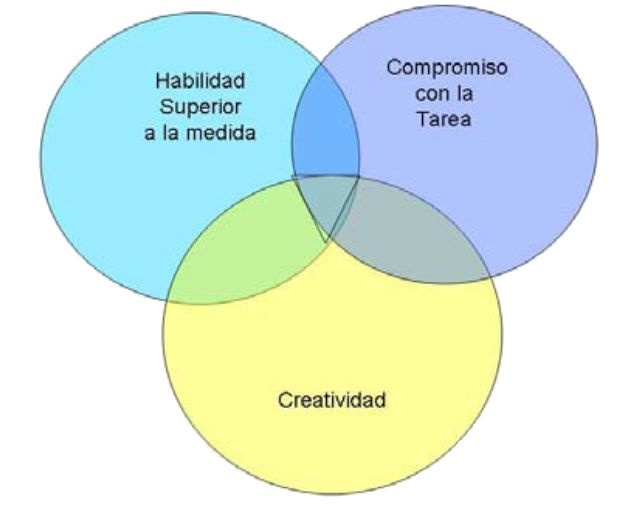
\includegraphics[width=0.55\textwidth]{img/renzulliVenn.png}
		\caption{Diagrama de Venn que ejemplifica la tríada que Renzulli acuñó en 1978 \parencite{reche2019models}. El primer anillo y el segundo son relativos a un alto nivel intelectual y a una creatividad elevada, respectivamente (Renzulli, 1978, citado en \citeauthor{Arocas2002OrientPsicopedGVA}, \citeyear{Arocas2002OrientPsicopedGVA}). El tercero habla del compromiso con la tarea (Renzulli, 1994, citado en \citeauthor{juntaAndaluciaManualAACC_2008}, \citeyear[9]{juntaAndaluciaManualAACC_2008})., que se operativiza mediante las definiciones de perseverancia, resistencia, práctica dedicada, confianza en sí mismo, etc. Finalmente el tercer anillo lo constituye una alta motivación de logro y persistencia
		en la tarea (Renzulli, 1978, citado en \citeauthor{Arocas2002OrientPsicopedGVA}, \citeyear{Arocas2002OrientPsicopedGVA}) .}
		\label{fig:renzulliVennEXTRETdeReche}
	\end{figure}
	\FloatBarrier
	
	\newpage
	\paragraph{\underline{Modelo de Gagné, 1985 (modelo diferenciado de dotación y talento)}}
	
	Este modelo distingue entre \textit{superdotación} y \textit{talento}. Así, habla de \textit{superdotación} cuando aparece una habilidad por encima de la media en \textbf{una o dos áreas} pertenecientes a las capacidades naturales o habilidades humanas; y de \textit{talento} cuando hay un rendimiento superior en\textbf{ uno o más campos} de la actividad humana \textcite{reche2019models}.
	
	
	\textcite{gagneModelBasatEnRendiment}, en su fuente primaria, en la página 89, especifica que estas habilidades o dominios son 4:
	
	
	\begin{itemize}[noitemsep]
		\item intelectual
		\item creativo
		\item socioafectivo
		\item sensoriomotor
	\end{itemize}
	
	El autor especificó en su momento que no acotaba más estas áreas dado que existieron diferencias importantes entre autores sobre qué subcategorias se pueden establecer para hablar de esos dominios (véase página 90 en el libro adjunto en \textcite{gagneModelBasatEnRendiment} consultado a través de research gate).
	
	
	

	
	
	
	
	
	\subsubsection{Modelos de orientación sociocultural}
	
	\paragraph{\underline{Tannenbaum, 1997} (Modelo psicosocial de los factores que componen la superdotación)}
	\label{par:tannenbaum}
	
	Este autor considera necesarios, además de la inteligencia, ciertos factores de personalidad, culturales y sociales. Considera fundamental la \textit{influencia ambiental a la hora de desarrollar el potencial de la persona} \parencite{reche2019models} pues, según él, \textit{la superdotación no puede ser definida
	fuera de un contexto social determinado} (Tannenbaum, 1986, citado en \citeauthor{Arocas2002OrientPsicopedGVA}, \citeyear{Arocas2002OrientPsicopedGVA}).
	
	Habla de cinco factores (figura \ref{fig:tannenbaumMonks}, izquierda):
	
	\begin{itemize}[noitemsep]
		\item Capacidad general.
		\item Aptitudes específicas.
		\item Factores no intelectuales (motivación, autoconcepto…).
		\item Influencias ambientales.
		\item Factor suerte.
	\end{itemize}
	
	 
	
	\paragraph{\underline{Monks, 1992 (Modelo de la interdependencia triádica)}}
	
	Monks revisa la teoría de Renzulli, considerando la sobredotación como un fenómeno dinámico o cambiante, resultante de la interacción del individuo con su entorno, añadiendo tres nuevas variables sociales que interactúan con las 3 variables consideradas por la teoria de Renzulli (las que vimos en la figura \ref{fig:renzulliVennEXTRETdeReche})). Estas son:
	
	\begin{itemize}[noitemsep]
		\item la familia
		\item los compañeros
		\item el colegio
	\end{itemize}
	 Estas 3 variables (ver figura \ref{fig:tannenbaumMonks}, derecha) interactúan con las tres variables que ya acuñó Renzulli en su modelo: la inteligencia, el compromiso con la tarea y la creatividad.
	
	
	\FloatBarrier
	\begin{figure}[htbp]
		\centering
		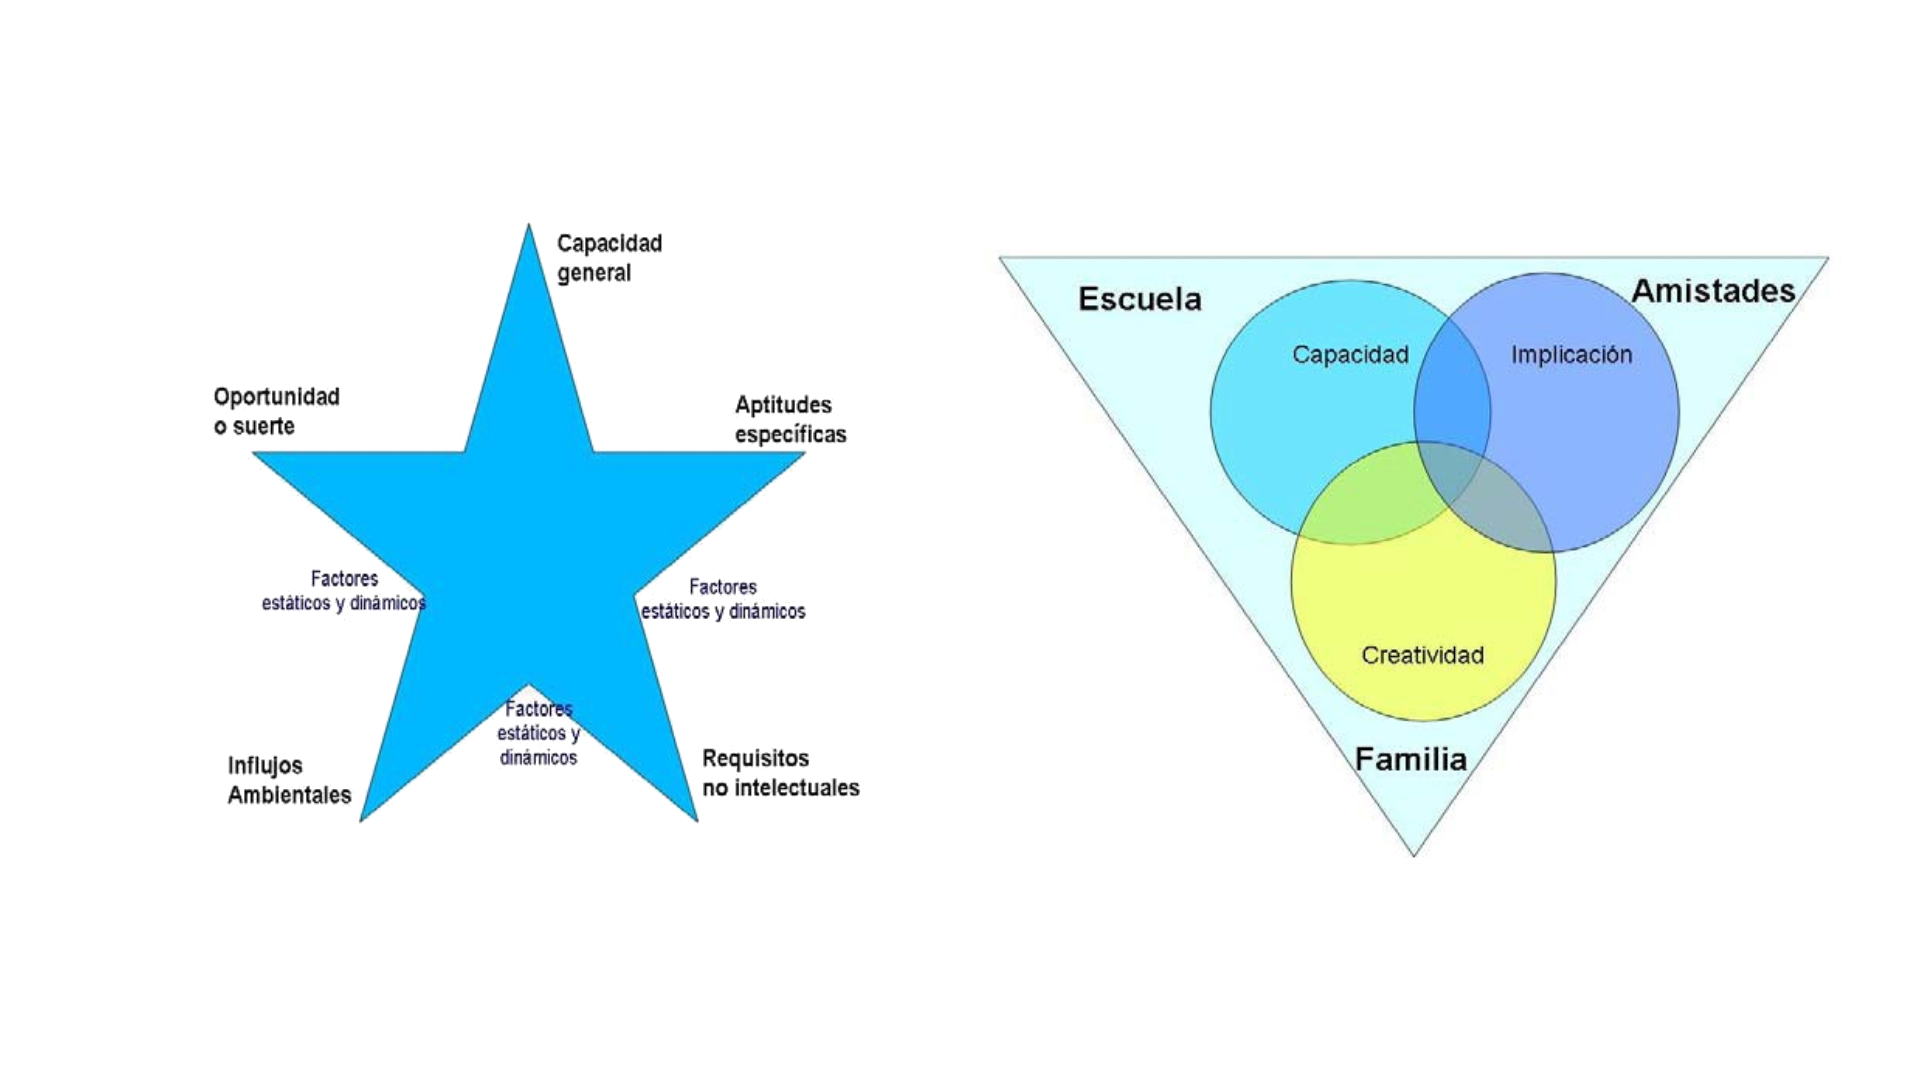
\includegraphics[width=1\textwidth]{img/TannenbaumMonks.png}
		\caption{Ilustración explicativa del modelo\textit{} de Tannenbaum (izquierda) y de Monks (derecha), extraidas de \cite{reche2019models}}.
		\label{fig:tannenbaumMonks}
	\end{figure}
	\FloatBarrier
	
	
	
	
	
	
	
	
	
	\subsubsection{Modelos cognitivos}
	
	En los modelos cognitivos, la investigación se orienta hacia productos
	tales como: medición de la inteligencia a través de tests, valoración de rendimiento, etc. Centran su interés en los procesos de de elaboración y gestión de la información \parencite{Arocas2002OrientPsicopedGVA}. Pretenden identificar los procesos y las estrategias que se ponen en marcha cuando se realizan tareas de un nivel superior \parencite{reche2019models}:
	
	\paragraph{\underline{Jackson y butterfield, 1986}} La capacidad metacognitiva superior es un componente fundamental de la superdotación \parencite{Arocas2002OrientPsicopedGVA}.
	
	\paragraph{\underline{Borowski y peck, 1986}} La metamemoria o autoconocimiento y autocontrol de la memoria es un determinante clave de la superdotación \parencite{Arocas2002OrientPsicopedGVA}.
	
	
	
	

	
	
	
	
	\paragraph{\underline{Stenberg, 1993 (Teoría triárquica de la inteligencia y pentagonal de la superdotación )}}
	
Este es el modelo \textit{\textbf{más representativo}} de los modelos cognitivos, según \textcite{reche2019models}, y propone explicar la superdotación conjugando altos niveles cognitivos, creatividad y una parte práctica, a saber:
	
	\begin{itemize}[noitemsep]
		\item \textbf{Subcategoría componencial:} Relaciones entre la inteligencia y el mundo interno de la persona. Procesos mentales implícitos en la inteligencia.
		\item \textbf{Subcategoría experiencial:} La inteligencia y su experiencia en el ciclo vital.
		\item \textbf{Subcategoría contextual:} La inteligencia y el mundo externo de la persona. Se refiere a los mecanismos que se usan en la adaptación, selección y configuración del medio.
	\end{itemize}
	
	
	También señala \textit{cinco criterios} que nos permiten poder hablar de altas capacidades:
	
	\begin{itemize}[noitemsep]
		\item \textbf{Criterio de excelencia:} Predominio superior en algún área o en varias.
		\item \textbf{Criterio de rareza:} Alto nivel de ejecución en algún aspecto excepcional.
		\item \textbf{Criterio de productividad:} Capacidad superior en el trabajo de algún campo específico.
		\item \textbf{Criterio de demostrabilidad:} La capacidad o capacidades se demuestran mediante pruebas válidas y fiables.
		\item \textbf{Criterio de valor:} La capacidad es reconocida y valorada por los demás.
	\end{itemize}
	
	
	
	
	
	
	
	
	
	
	
	
	
	\subsubsection{Modelos basados en capacidades}
	
	Estos modelos son los modelos clásicos, otorgar una importancia
	casi exclusiva a la \textbf{inteligencia general} y al \textbf{cociente intelectual}. Progresivamente se van considerando
	otras capacidades específicas o talentos  \parencite{Arocas2002OrientPsicopedGVA}:
	
	
	\paragraph{\underline{Terman (1917)}}
	
	De acuerdo con \textcite{Arocas2002OrientPsicopedGVA}, uno de los materiales para esta actividad oblgatoria, Terman es el autor \textit{más representativo} de este enfoque. Sus aportaciones se centraron en
	medir la \textit{inteligencia general} utilizando los instrumentos y conocimientos científicos de su tiempo (Stanford-Binet, Spearman, Stern, etc.). \textbf{Estableció el criterio de selección de las personas superdotadas \textit{en un C.I. superior a 140}}, criterio que ha perdurado en el tiempo y que, a día de hoy, todavía es considerado por algunos profesionales y publicaciones.
	
	\paragraph{\underline{Marland, 1972 (revisión del enfoque de Terman)}} De acuerdo con \textcite{Arocas2002OrientPsicopedGVA}, el grupo de colaboradores de Terman refinó la concepción inicial añadiendo más complejidad al concepto de superdotación. La U.S. Office of Education
	(U.S.O.E.) de Estados Unidos\textbf{ aceptó en el 72 su concepción de los niños superdotados} y con talentos \textbf{como aquellos} que por sus habilidades extraordinarias son \textbf{capaces de altas realizaciones} e incluyó a los que poseían \underline{alguna} de estas características:
	
	\begin{itemize}[noitemsep]
		\item Alta capacidad intelectual general.
		\item Aptitud académica específica.
		\item Pensamiento creativo o productivo.
		\item Habilidad de liderazgo.
		\item Habilidad en artes visuales o representativas.
		\item Habilidad psicomotriz.
	\end{itemize}
	
	NOTA: El congreso eliminó de esta clasificación la habilidad psicomotriz en 1978.
	
	\begin{tcolorbox}[
		colback=gray!10,
		colframe=gray!50,
		boxrule=0.5pt,
		arc=2mm
		]
		\textit{\textbf{NOTA}}: El congreso eliminó de esta clasificación la habilidad psicomotriz en 1978 \parencite{Arocas2002OrientPsicopedGVA}
	\end{tcolorbox}
	
	\paragraph{\underline{Howard , 1984 - 1985 (modelo inteligencias múltiples)}}
	\label{par:modelosCapacidades}
	
	Este autor cambia la concepción de la inteligencia, que con él deja de ser un elemento único y estático. Además, pretende tener presente toda la variedad de capacidades cognitivas.
	
	De acuerdo con Torrego (2011, citado en \citeauthor{reche2019models}, \citeyear{reche2019models}) y con Gardner (1985, citado en \citeauthor{Arocas2002OrientPsicopedGVA}, \citeyear{Arocas2002OrientPsicopedGVA}) bajo este marco se nos habla de siete tipos de inteligencia -o incluso ocho (\underline{ver nota, es importante}\footnote{Cuidado porque en la referencia de \textcite{Arocas2002OrientPsicopedGVA}, donde se cita a Gardner en 1985, se incluye entre estas 7 inteligencias la inteligencia Musical pero NO se cita la Naturalista; mientras que en la referencia de \textcite{reche2019models}, que cita a una referencia de Gardner del 1984 -un año antes- pasa al revés: se cita la Naturalista pero no la Musical. Desconozco la razón de la permuta, y si esta es un error de alguna de las dos referencias secundarias o, por el contrario, Gardner decidió cambiar una por otra en el transcurso de un año.})-, a saber:
	
	\begin{enumerate}
		\item \textbf{Lingüística-verbal}: Es la capacidad de usar el lenguaje de manera efectiva, en forma oral o escrita. Incluye varias habilidades necesarias para el lenguaje (sintaxis, fonética, semántica\dots). Los alumnos en los que predomina esta inteligencia destacan en la lectura, escritura, narración de historias, etc.
		
		
		\item \textbf{Lógica-matemática}: Es la capacidad que tiene una persona para usar los números de manera eficaz y de razonar de una manera adecuada. Los alumnos destacarían en matemáticas, resolución de problemas, razonamiento lógico...
		
		\item \textbf{Espacial}: Capacidad para pensar en tres dimensiones, reconocer la forma, el espacio, el color, etc. Dicha capacidad permitiría a una persona retener imágenes y trabajar con ellas mentalmente: transformándolas, modificándolas, analizándolas. Los alumnos con predominio de este tipo de inteligencia destacan en puzles, lectura de gráficos, imaginación, etc.
		
		\item \textbf{Corporal-kinestésica}: Se trata de la capacidad para usar el cuerpo como medio para expresar ideas y sentimientos; así mismo, presenta habilidades de coordinación, equilibrio y flexibilidad. Los alumnos destacan en educación física, en trabajos manuales, representaciones corporales.
		
		\item \textbf{Naturalista}: Esta referencia se cita \textit{solamente} en Torrego (2011, citado en \citeauthor{reche2019models}, \citeyear{reche2019models}), \textit{pero no} en Gardner (1985, citado en \citeauthor{Arocas2002OrientPsicopedGVA}, \citeyear{Arocas2002OrientPsicopedGVA}) Saben distinguir, clasificar y utilizar elementos del medio ambiente, objetos, animales y plantas. Destacan en habilidades como la observación, experimentación y reflexión.
		
		\item \textbf{Musical}: Esta referencia se cita solamente en Gardner (1985, citado en \citeauthor{Arocas2002OrientPsicopedGVA}, \citeyear{Arocas2002OrientPsicopedGVA}); \textit{pero no} en Torrego (2011, citado en \citeauthor{reche2019models}, \citeyear{reche2019models}). La inteligencia Musical se define como la capacidad para percibir, distinguir, transformar y expresar las formas musicales. Esta inteligencia incluye la sensibilidad al ritmo, el tono, la melodía y el timbre de una pieza musical, permitiendo a los individuos comunicarse y comprender el mundo a través del sonido Gardner. El sujeto puede tocar un instrumento, darse cuenta de sonidos no verbales en el ambiente, aprender con más facilidad si canta, etc. Gardner (1983, citado en \citeauthor{piperMusicalIntelligence}, \citeyear{piperMusicalIntelligence}). \textbf{Véase nota al pie}\footnote{Se intentó encontrar la referencia original de 1983 en scopus pero no se encontró, solo se pudo acceder a otro estudio de Gardner en el que no conceptualizaba de cero la inteligencia musical y, además, no tenía el full text accesible (véase la imagen aquí \ref{fig:gardnerIntent}).}. \textit{Considerar este tipo de inteligencia, a título personal, me parece muy relevante dado que se sabe que aprender a tocar un instrumento tiene una correlación con mejores puntuaciones académicas; de ahí que en china se investigue el rol de las habilidades musicales  \parencite{multiplesInteligenciesMusicaXinaSCOPUS}.}
		
		\item \textbf{Interpersonal}: Buena capacidad para mostrar empatía por los demás, entendiendo e interaccionando adecuadamente con ellos.
		
		\item \textbf{Intrapersonal}: Es la habilidad y capacidad de construir una percepción precisa respecto a uno mismo y de organizar y dirigir su propia vida. Se tienen presentes aptitudes como la autodisciplina, la autocomprensión y la autoestima.
	\end{enumerate}
	
	
	
	
	% --------------------------
	\subsection{Características cognitivas, socioemocionales y educativas del alumno con alta capacidad.}
	
	El alumnado con altas capacidades intelectuales destaca por su flexibilidad cognitiva, mayores habilidades
	metacognitivas, \textbf{velocidad en la adquisición y procesamiento de la información}, uso del lenguaje, niveles
	de persistencia, pero también una \textbf{alta sensibilidad emocional y sensorial} y
	potencial creativo \parencite[9]{gobiernoVascoPlanAACC2019_recomanatUned}
	
	
	
	
	% --------------------------
	\subsection{Factores que influyen en la identificación y desarrollo del alumno con alta capacidad}
	
	
	De acuerdo con \parencite[10]{Arocas2002OrientPsicopedGVA}, la \textbf{identificación del alumnado con superdotación} es un tema complejo y polémico, principalmente
	dentro del campo educativo, dado que hay partidarios y detractores de la conveniencia de su identificación.
	
	Los \textbf{partidarios de la mencionada identificación} lo justifican desde varios puntos de vista: desde el \textit{punto de vista \underline{sociopolítico}}, por las aportaciones y beneficios que pueden dar ellos a la sociedad y al país; pero también desde el \textit{punto de vista \underline{educativo}}, dado que puede dar lugar a una respuesta educativa que \textit{desarrolle al máximo las potencialidades}, por un lado, y \textit{evite su fracaso escolar}, por el otro \parencite[10--11]{Arocas2002OrientPsicopedGVA}.
	
	Además en comunidades autónomas como el País Vasco solo el 32,8 y el 25,4 por ciento de las direcciones educativas de colegios de primaria y secundaria, respectivamente, disponían de planes para detección de altas capacidades hace siete años \parencite[20]{gobiernoVascoPlanAACC2019_recomanatUned}. Estos porcentajes subieron entonces a 67,2 i 50,2 por ciento en educación infantil y bachillerato, que es, en mi opinión, claramente insuficiente.
	
	
	
	En esta misma comunidad hay en los \underline{últimos años} \textbf{una mejora \textit{aparente}}, pues se declara que el porcentaje general -sin discriminar por etapas- ha subido al 90 por ciento \parencite[65]{gobiernoVascoEstrategia2024}. A título personal, considero que esta mejora es \textit{aparente} dado que no se dan tantísimos datos como antes, y con ello no podemos vislumbrar un interés real en que los centros atiendan este tipo de alumnado específicamente. El informe que el gobierno Vasco publica actualmente sobre el tema de las altas capacidades NO está tan siquiera dirigido a altas capacidades específicamente como sí lo estaba antes, sino que engloba todas las necesidades educativas especiales. En mi opinión, no hacer un informe específico sobre la materia es un menoscabo a la atención a la parte derecha de la curva normal que, justamente, obedece a opiniones políticas.
	
	
	% --------------------------
	\subsection{Relación entre altas capacidades y riesgo de exclusión educativa o social}
	
	Como se comentó en \textcite[10--11]{Arocas2002OrientPsicopedGVA} una de las finalidades de detectar a los alumnos con altas capacidades es evitar su fracaso escolar.
	
	Fracasar escolarmente, naturalmente, incrementa el riesgo de quedar excluido socialmente. Si un alumno de secundaria deja los estudios no puede incorporarse al mercado laboral hasta los 16 años, y queda en un limbo hasta esa edad. En países de hispanoamérica, los alumnos que no tienen apoyo pueden caer en pandillas y en España, aunque este riesgo sea mucho más reducido, la pérdida de habilidades de un alumno con alto potencial seria plausible e irreversible. Además, es bien sabido que contar con un mayor nivel educativo es una protección contra el desempleo en nuestro país y, también, contra los salarios bajos \parencite{bbvaSalarioEstudios}.
	

	
	
	
	
	
	
	% --------------------------
	\subsection{Inclusión Educativa: Explicación de cómo el concepto de inclusión educativa se relaciona con la equidad y la ciudadanía en el ámbito escolar. ¿Principales desafíos para su implementación en los centros educativos? Justificar con bibliografía básica de la asignatura.}
	
	
	La respuesta al alumnado con altas capacidades intelectuales sigue necesitando un impulso por parte de todos los agentes de la comunidad educativa en términos de inclusión y es necesaria la formación en el profesorado, tanto inicial como permanente \parencite[9]{gobiernoVascoPlanAACC2019_recomanatUned}.
	
	Además, la atención educativa al alumnado con altas capacidades intelectuales debe de contar con un
	plan específico, que recoja las prioridades a desarrollar a corto y medio plazo de acuerdo con el \textcite[10]{gobiernoVascoPlanAACC2019_recomanatUned}. Cosa que en mi opinión, al menos en el país Vasco, \underline{no se está haciendo} porque el informe más reciente del \textcite{gobiernoVascoEstrategia2024}, como se ha comentado, no es específico ni focaliza en las altas capacidades.

	
	
	
	
	
	
	
	
	
	
	
	
	% --- Parte 4: Marco Teórico (2-4 páginas)
	\newpage
	\section{Diseño de evaluación por sospecha de presentar necesidades específicas de apoyo educativo (NEAE) asociadas a Altas Capacidades}
	

	
	\subsection{Nombrar la normativa vigente en mi comuidad autópnoma y objeto de la misma (identificacion, establecimiento de medidas, etc)}
	

		
	El marco normativo y pedagógico en Cataluña para el abordaje de las altas capacidades intelectuales se fundamenta en el paradigma de la educación inclusiva establecido por el DECRET 150/2017 \parencite{decret150_2017}. En este texto jurídico encontramos, en su artículo 5, la cita literal ``\textit{e) Els alumnes amb altes capacitats derivades de la superdotació intel·lectual, els talents simples i complexos i la precocitat}'' que significa ``\textit{e) los alumnos con altas capacidades derivadas de la sobredotación intelectual, talentos simples, complejos y la precocidad}''.
	
	
	 También se debe hacer mención a la resolución ENS/1543/2013 \parencite{resolucioENS1543_2013} y a otras guías de referencia que probablemente emanan de la misma, y son más comprensivas: por un lado  \textcite{xtecAltesCapacitats} y, por el otro \href{https://educacio.gencat.cat/web/.content/home/departament/publicacions/colleccions/inclusio/altes-capacitats/altes_capacitats.pdf}{\textcite{gencatAltesCapacitats2013}}), en formato manual. Textos que pueden guiar el día a día de los profesionales. 
	 
		\begin{tcolorbox}[
	 			colback=gray!10,
	 			colframe=gray!50,
	 			boxrule=0.5pt,
	 			arc=2mm]
			\textbf{NOTA:} \textit{se ha puesto hipervínculo directo en la referencia bibliográfica dispuesta tres líneas arriba para que el lector pueda ir del texto de esta actividad directamente a a la guía sin tener que pasar por referencias.}
		\end{tcolorbox}
	  \underline{La identificación de este alumnado} se entiende como un proceso continuo y colaborativo que va más allá de una simple administración de pruebas psicométricas. Este procedimiento se inicia con la \textbf{detección de indicadores de talento o superdotación en los entornos escolar y familiar}, terminando \textbf{en una evaluación psicopedagógica exhaustiva por parte del Equipo de Asesoramiento y Orientación Psicopedagógica (EAP)}, organismo encargado de determinar las necesidades específicas de apoyo educativo \parencite[15]{gencatAltesCapacitats2013}. En mi experiencia como orientador, empero, el EAP solamente interviene cuando existen fundamentos claros de altas capacidades y/o, a veces, disrupción en el ámbito educativo (algo que, para mí, es mejorable porque fomenta que no exista una elevada sensibilidad en la detección de las altas capacidades en caso que el alumno se integre bien en el grupo clase).
	
	 \underline{Una vez identificado el alumno con AACC}\footnote{AACC será la denominación que se usará en el resto del trabajo para referirse a altas capacidades}, se prioriza \textbf{la aplicación de medidas en el aula ordinaria}, promoviendo la flexibilización metodológica o el enriquecimiento curricular, que deben documentarse a través de lo que llaman el ``\textbf{Plan Individualizado}'' (PI). Finalmente, en aquellos casos donde el enriquecimiento mencionado no logre dar una respuesta ajustada al desarrollo del alumno, la normativa permite la aplicación de medidas \textbf{excepcionales} y más drásticas, como llevar a cabo la ``\textit{flexibilización de la permanencia en un curso, en un ciclo o en toda la etapa educativa}''\parencite[4]{resolucioENS1543_2013}\footnote{Cita literal: ``que l’escolarització dels alumnes amb altes capacitats intel·lectuals podrà comportar tant l’adaptació curricular com la flexibilització de la permanència en un curs, en un cicle o en tota l’etapa educativa''}.
	 
	 
	 
	 	\subsection{medición psicométrica de las altas capacidades}
	 	\label{subsec:medicionPsicometrica}
			 	
			\begin{tcolorbox}[
				colback=gray!10,
				colframe=gray!50,
				boxrule=0.5pt,
				arc=2mm
			]
			Por simplicidad, en este subapartado se han englobado los tres subapartados de la plantilla para la elaboración del trabajo, a saber:
			
			\begin{itemize}
				\item ``presentar las variables básicas a valorar en estas evaluaciones por parte de los servicios de orientación''.
				\item ``tipos de instrumentos a utilizar por cada variable''. 
				\item ``nombrar pruebas psicopedagógicas, cuestionarios para las variables principales y puntos de corte que indicarían Altas Capacidades''.
			\end{itemize}

		\end{tcolorbox}

	 	
	 	
	 	
	 Los servicios de orientación de los centros solo disponen de autoinformes, las valoraciones más profundas y el diagnóstico los hacen los equipos de atención psicopedagógica (no cito referencia, porque tengo un año de experiencia trabajando como orientador y he abordado derivaciones de casos de dislexia y visto abordajes de casos de AACC\footnote{En Cataluña, desde la pandemia, se permitió inscribirse a la bolsa de profesorado de secundaria sin tener el máster, con el compromiso de obtenerlo.}). 
	 
	 Los servicios de orientación sí pueden hablar con la familia y el profesorado para determinar si existen indicios de AACC. Esto se hace mediante las herramientas de observación que tienen que rellenar padres y maestros (para los más pequeños) a modo de procedimiento informal, previo a la actuación del EAP 	 \parencite[11]{gencatAltesCapacitats2013}:
	 
	 \begin{itemize}[noitemsep]
	 	\item cuadros de observación para el profesorado.
	 	\item cuadros de observación para padres.
	 	\item  autoinforme de los alumnos en educación secundaria.
	 \end{itemize}
	 

	 
	  Luego, después de que el equipo de orientación del centro pase estas informaciones, si los indicios son claros, será el EAP que deba utilizar no solamente el coociente intelectual (CI) si no tambien evaluar si en otros contextos se vislumbran las altas capacidades
	  \parencite[p.~10, párr.~3]{gencatAltesCapacitats2013}. Esto se hace así porque los EAPs tienen recursos limitados y no pueden valorar, en la práctica, toda la complejidad y necesidades educativas especiales que se ven en las aulas (en mi caso, trabajando en un centro de la zona del norte de Catalunya, el mismo profesional del EAP con el que me reunía quincenalmente dijo que no iba a hacer más de una valoración de dislexia en lo que quedaba de curso).
	  
	  Los instrumentos a utilizar a nivel informal antes del EAP, para los alumnos de la ESO, incluyen múltiples items. No podría decir todas las variables que valoran por su extensión, pero se trata de una escala de tipo likert con 30 items, que trata de sistematizar qué ven el profesorado y los familiares sobre el alumno y, también, el propio alumno de sí mismo \parencite[21]{gencatAltesCapacitats2013}: si el adolescente se relaciona con alumnos mayores, si se organiza de forma que tiene tiempo para hacerlo todo, si su vocabulario es rico para su edad, si se aburre en clase, si tiene alta capacidad para transferir con facilidad los aprendizajes a otras situaciones, etc. \parencite[19]{gencatAltesCapacitats2013}. 
	  
	  
	  Podéis ver una parte\textbf{de los 30 items} de esta tabla en la figura \ref{fig:graellaValorAACC914anys}, de la tabla que se administra a profesores y/o familiares. Cuando la puntuación directa de la tabla, organizada como items en base likert de 1 a 5 puntos por item, da superior a \textbf{70 puntos} es cuando hay indicios para precisar que un especialista de EAP haga una \textbf{valoración psicopedagógica} yconfirme el diagnóstico de AACC \parencite[29]{gencatAltesCapacitats2013}, siempre que el tutor de su grupo nos dé el visto bueno \parencite[p.37, punto 1]{gencatAltesCapacitats2013}.  Por lo tanto, este sería el primer punto de corte que encontraremos en la evaluación por sospecha de un alumno de AACC.
	  
	  Es muy interesante ver que en Catalunya los orientadores de los centros también disponemos de\textbf{ otra tabla o graella de valoración}, que \textbf{mapea casi de forma unívoca los distintos apartados a evaluar con las distintas inteligencias que teorizó Howard Gardner mediante su modelo de inteligencias múltiples}  (véase de nuevo el apartado  \ref{par:modelosCapacidades}, de modelos basados en capacidades). Esta tabla la podéis ver en \parencite[22--24]{gencatAltesCapacitats2013} y también, en versión muy reducida, en la figura \ref{fig:graellaValorAACCGARDNER}. Es menester mencionar, que en esta tabla se incluyen 9 tipos de inteligencias a valorar, no las 8 que tenía la teoria original: como curiosidad, tenemos una más: la inteligencia espiritual \parencite[24]{gencatAltesCapacitats2013}.
	  
	   A parte de esta última tabla, se encuentra otra tabla también dirigida para valorar inteligencias múltiples, pero esta vez por parte de familias y profesores \textcite[26-28]{gencatAltesCapacitats2013}.
	
	
	\FloatBarrier
	\begin{figure}[htbp]
		\centering
		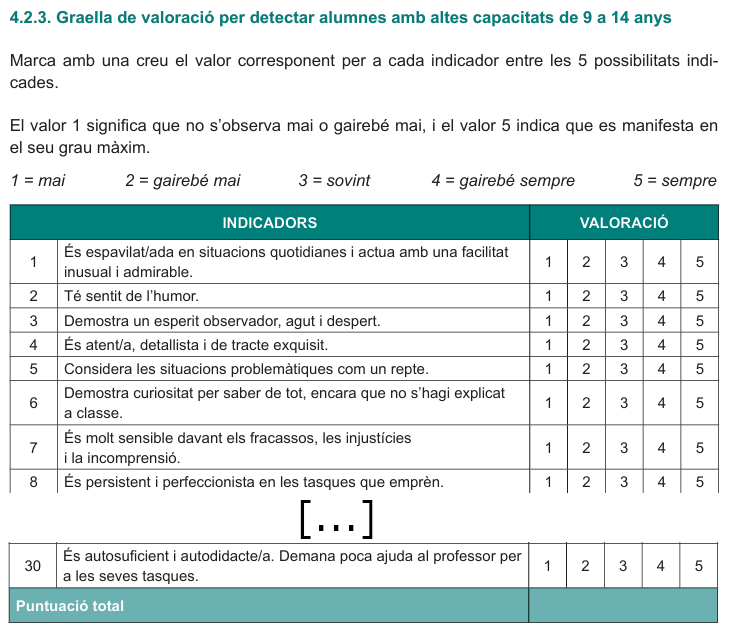
\includegraphics[width=1\textwidth]{img/graellaValoracio914anys.png}
		\caption{Fragmento de una tabla de valoración informal para familia y profesores. Es lo que aplican los orientadores educativos al profesorado y/o a las famílias para poder justificar su derivación posterior a EAP (lo he visto en la práctica profesional). Tabla extraída de \textcite[19]{gencatAltesCapacitats2013}}
		\label{fig:graellaValorAACC914anys}
	\end{figure}
	\FloatBarrier
	
	
	\FloatBarrier
	\begin{figure}[htbp]
		\centering
		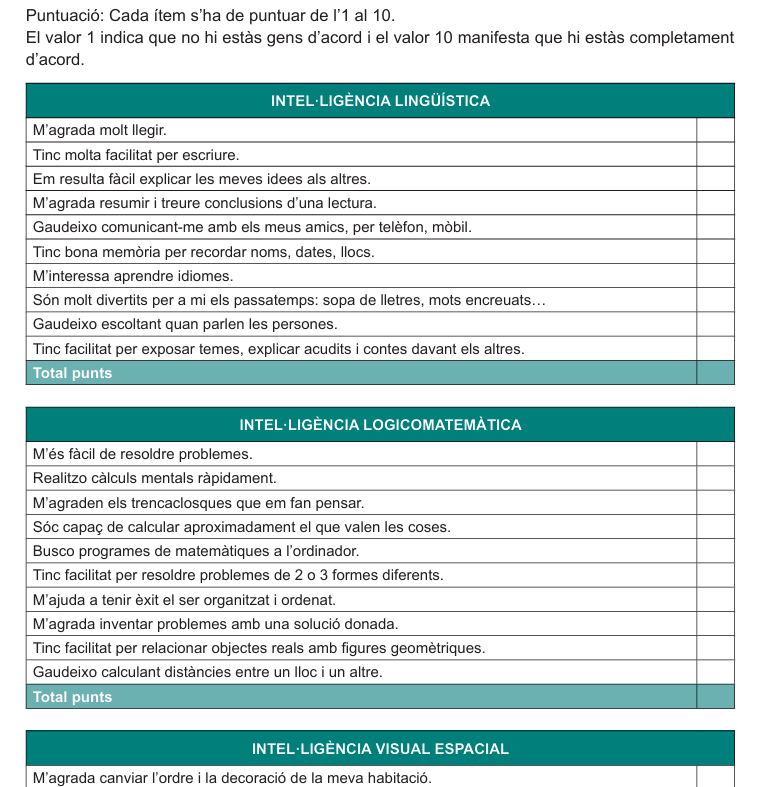
\includegraphics[width=1\textwidth]{img/graellaValoracioGardner.png}
		\caption{Fragmento de una tabla de valoración informal para alumnos, para hacer un autoinforme inteligencias múltiples según el modelo de Gardner. Fragmento de la tabla extraída de \textcite[22]{gencatAltesCapacitats2013}.}
		\label{fig:graellaValorAACCGARDNER}
	\end{figure}
	\FloatBarrier
	
	
	Ya por terminar este apartado, quedaría mencionar someramente las pruebas psicométricas y observaciones que puedan hacer en el equipo de atención psicopedagógica. No entraré en hacer una valoración detallada dado que el apartado pide hacer un ``\textit{diseño de evaluación por sospecha}'' y no un ``\textit{diseño de evaluación exhaustivo}''. Entiendo que su objetivo no persigue entrar a describir las pruebas psicométricas al nivel de detalle al que entraría un profesional de EAP, así que solo mencionaré lo que he podido ver en mi práctica profesional.
	
	Durante mi año de experiencia trabajando como orientador, he visto que se utiliza, principalmente, la escala de Weschler como pruebas objetivas psicométricas. Para niños se utiliza el Wisc-IV y para adultos el WAIS. La escala de Wechler considera sobredotación intelecutal en términos de coociente intelecutal (tomando solamente el criterio del CI, que sabemos que no es el único) como estar 2 desviaciones típicas por encima de la media. En adultos, al menos en el caso de la distribución del WAIS-III que es la que conocí cuando estudié, tiene media 100 y desviación típica 15: ello supone que un adulto valorado con esta distribución de datos y escala, si obtuviera más de 130 de CI se consideraría por encima del umbral de la sobredotación. Probablemente el WISC siga unos estándares parecidos.
	
	
	
	
	% parte5: V. Diseño de la Intervención ((-5 páginas))
	\newpage
	\section{Diseño de la Intervención}
	
	caso escogido $\rightarrow$ \textbf{\underline{Caso 2}: Alumno de 1o de la ESO.}
	
	
	
	
		\begin{tcolorbox}[
			colback=gray!10,
			colframe=gray!50,
			boxrule=0.5pt,
			arc=2mm
		]
		
		\textbf{Caso 2}: Alumno de 1r curso de la ESO identificado con Altas Capacidades en 5º de Primaria a raíz de problemas de conducta, entre ellos, una marcada intolerancia ante errores propios y ajenos. Presenta un rendimiento académico medio, excepto en matemáticas, donde destaca de manera excepcional. Tiene dificultades en la relación con sus iguales y muestra una actitud desafiante hacia los adultos. Dedica gran parte de su tiempo a la compañía de un tío experto en física cuántica. Aunque no manifiesta un interés académico significativo, no suspende ninguna asignatura. Su identificación surgió a partir de una evaluación inicial por problemas de conducta, que posteriormente confirmó su perfil de Alta Capacidad. De manera autodidacta, ha aprendido a tocar la guitarra y el piano, además de componer música.

		\end{tcolorbox}

	
	
	
	
	
	
	
	
	
	
	
	Para diseñar la intervención vamos a tomar los intrumentos que ya hemos mencionado en el apartado \ref{subsec:medicionPsicometrica} de medición psicométrica. Al final estamos en la comunidad autónoma de Cataluña y existen unos protocolos que no nos podemos saltar.
	
	Podemos decir que el marco teórico que nos fuerza a seguir estos protocolos de detección inicial es una mezcla entre la teoria de inteligencias múltiples de Gardner (véase \ref{par:modelosCapacidades}), por las tablas que tenemos que pasar que básicamente implementan su teoría \parencite[pp. 22--24 y 26 -- 28]{gencatAltesCapacitats2013} que ya vimos en el subapartado anterior; y varios de los distintos modelos que hemos visto en el apartado del marco teórico, y cuyas ideas se subliman en el cuestionario de los 30 items que mencionamos \parencite[19]{gencatAltesCapacitats2013}.
	
	En ese cuestionario (véase de nuevo la figura \ref{fig:graellaValorAACC914anys}) se implementa en algunos ítems los tres constructos que vio necesarios Renzulli en su modelo basado en el rendimiento (véase \ref{par:renzulli}): la curiosidad, medido por ejemplo por el \textit{ítem 6} del cuestionario; y la persistencia en la tarea, por el \textit{ítem 8} de la tabla de valoración. En ese cuestionario también se implementan características del modelo sociocultural que acuñó Tannenbaum en 1997 (véase \ref{par:tannenbaum}), que sostenía que no se pueden darse las AACC fuera de un contexto social determinado  (Tannenbaum, 1986, citado en \citeauthor{Arocas2002OrientPsicopedGVA}, \citeyear{Arocas2002OrientPsicopedGVA}) ni de una influencia ambiental adeduada para poder desarrollar su potencial \parencite{reche2019models} -de ahí quizás la presencia del \textit{ítem 11} de la tabla que pregunta por si el niño prefiere relacionarse con personas mayores a él-, etc.
	
	Para mí, hay algo que salta a la vista y que hay que indagar: gran parte de las características descritas por los modelos mencionados, en este niño, parece ser que se dan a la perfección. La curiosidad y la persistencia en la tarea se pueden ver en sus ganas de aprender a tocar dos instrumentos (¡solo!) y luego, el contexto social determinado y enriquecido que teorizaba Tannenbaum, parece ser que también se da: el hecho de que el alumno dedique gran parte de su tiempo a la compañía de un tío experto en física cuántica nos indicaría, según este último modelo, que el niño tendría el ``andamiaje'' adecuado para poder pavimentar una carretera hacia las altas capacidades. 
	
	Sin embargo, sería bueno corroborar si su tío realmente es quien dice ser. Es decir, si realmente es un experto en física cuántica, significa que tendría un doctorado en la materia; pero también podría ser que no fuera el caso y que de física cuántica solo tuviera una noción a nivel divulgativo. También habría que valorar el desempeño con los instrumentos y su capacidad de aprendizaje. Sí llama la atención su facilidad para aprobar sin mostrar interés académico y su rendimiento excepcional en matemáticas lo cual, para mi, es un indicio suficiente para iniciar una intervención.
	
	La propuesta de intervención sería pasar las tablas mencionadas a familia, profesores y alumno. Acto seguido, si da los cortes adecuados y supera los umbrales de los baremos dados por la generalitat, derivarlo al EAP; pero eso sí, previamente teniendo el consentimiento del tutor del grupo al que pertenece, de la dirección del centro (el director es el que tiene la última palabra), de acuerdo con \textcite[19]{gencatAltesCapacitats2013} y también de la família por escrito (véase la hoja de consentimiento \textcite[38]{gencatAltesCapacitats2013}). Yo mismo, en mi práctica profesional, tuve que hacer la valoración de dilexia de dos alumnos mediante tablas prediseñadas por la generalitat y tuve que aplicar todos estos pasos antes de poder hacer la derivación a EAP.
	
	
	
	
	
	
	
	
	% parte 6: 1 pàgina
	\newpage
	\section{Conclusiones}
	
	
	Esta actividad ha sido verdaderamente mucho más últil de lo que me pensaba antes de empezarla. 
	
	En primer lugar, me pude volver a empapar de modelos teóricos de la sobredotación intelectual que ya tenía olvidados; porque solo los vi de pasada en asignaturas que hice hace más de 10 años. La teoría de los mismos es fundamental para entender el por qué unos cuestionarios institucionales del \textit{departament d'educació} están diseñados de la forma como están.
	
	En segundo lugar, la mayor utilidad de la actividad, sin duda alguna, ha sido obligarme a ver los protocolos de actuación para mi comunidad autónoma. Si bien estoy familiarizado con los protocolos de detección iniciales que fija la comunidad autónoma y derivación posterior a EAP, solo para alumnos con sospecha de dislexia y trastorno leve del aprendizaje, nunca jamás había tenido que hacer yo una derivación a EAP de un alumno que se sospecha que tiene altas capacidades.
	
	Cada caso de necesidades educativas especiales tiene sus propios protocolos de actuación y esta actividad y su caso práctico me han permitido \textbf{aprender} algo que me podrá ser muy útil en los años venideros, porque ahora ya sé dónde encontrar esta información.
	
	Además, ha sido la excusa perfecta para volver a utilizar el sistema de software libre LaTeX y su paquete de gestión bibliográfica en APA de la séptima edición, utilizando Bibtex y volviendo a tener un contacto con mi parte académica. He de admitir que el trabajo de campo en el ámbito educativo estaba empezando a hacer que perdiera la reflexión y el aprendizaje en pro de actuar rápido y en base a la forma que tiene de actuar cada centro. Es importante tener conocimientos que trasciendan la organización de cada centro, para saber también implementar mejoras a futuro en los centros donde se trabaje y/o anticiparse a las necesidades de cada uno.
	

	
	
	
	
	
	\clearpage
	% --- Referencias Bibliográficas ---
	\printbibliography[title={Referencias Bibliográficas}]
	
\end{document}